\chapter{Интеллектуальные системы регистрации и анализа проблемных ситуаций, возникающих в ИТ-инфраструктуре предприятия} \label{chapt1}

\section{Сравнительный анализ систем регистрации и устранения проблемных ситуаций} 
В данной главе рассматриваются имеющиеся на данный момент интеллектуальные системы регистрации и анализа проблемных ситуаций. \par
\textbf{HP OpenView} \cite{HPOpenView} \cite{HP1} \cite{HP2} \cite{HP3} является комплексным программным решением по мониторингу ИТ-инфраструктуры предприятия и имеет множество модулей. На рисунке \ref{img:hpopenview} представлен вид системы, которая обладает широким спектром возможностей: мониторинг \cite{HP4} \cite{HP5}; регистрация инцидентов; управление системами. Система не поддерживает: понимание и формализацию запросов; автоматическое исправление проблемы на основе формализации запроса.

\begin{figure} [h] 
  \center
  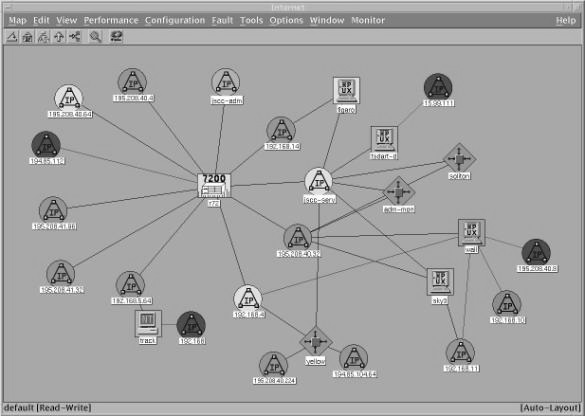
\includegraphics [scale=1.0] {hpopenview}
  \caption{HP OpenView} 
  \label{img:hpopenview}  
\end{figure}

Система \textbf{ServiceNOW}~--- средства автоматизации сервиса. На рисунке \ref{img:svnow} представлен вид этой системы, которая предоставляет следующие возможности: регистрация инцидентов и создание цепи их обработки. Система не поддерживает: понимание и формализацию запросов; автоматическое исправление проблемы на основе формализации запроса. Система широко используется в ИТ-инфраструктуре CERN \cite{SN1} \cite{SN2} для регистрации инцидентов и их решения.

\begin{figure} [h] 
  \center
  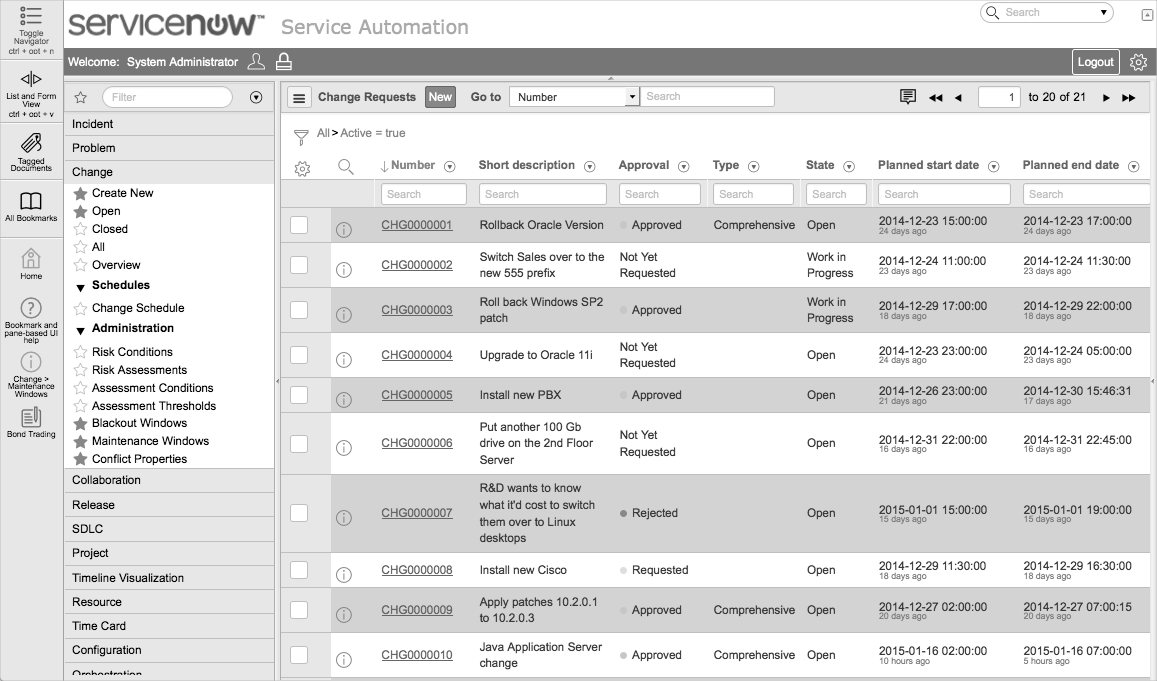
\includegraphics [scale=0.3] {svnow}
  \caption{Service NOW} 
  \label{img:svnow}  
\end{figure}

\textbf{IBMWatson}~--- это вопросно-ответная система, которая поддерживает: понимание и формализацию запросов и поиск решений. Система не поддерживает автоматическое исправление проблемы на основе формализации запроса. Система широко используется в медицине для постановки диагнозов болезней \cite{IBM1} \cite{IBM2} \cite{IBM3} \cite{IBM4} и реализует базовые принципы искусственного интеллекта \cite{IBM5} \cite{IBM6}. Ее разработка велась под суперкомпьютер IBM Deep Blue \cite{IBM7}. На рисунке \ref{img:Watson-Analytics} представлен общий вид этой системы. \par


\begin{figure} [h] 
  \center
  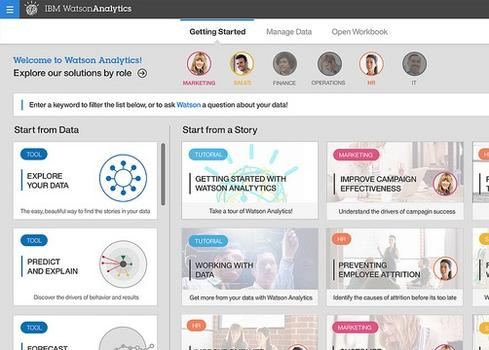
\includegraphics [scale=1.0] {Watson-Analytics}
  \caption{Пример работы системы Watson} 
  \label{img:Watson-Analytics}  
\end{figure}

Кроме того, известны следующие дополнительные способы и системы автоматизации:
\begin{itemize}
	\item Обработка инцидентов посредством регулярных выражений. В таком решении нет гибкости, так как обработка идет путем поиска ключевых слов вне контекста. Метод регулярных выражений частично используется для обработки естественного языка, поиска  \cite{REG1}, диагностики активных систем \cite{REG2}, анализа поведения функций \cite{REG4}, обработки данных в системе eDiscovery \cite{REG5}, в разработке способах программирования \cite{REG3};
	\item Обработка инцидентов при помощи скриптов~--- автоматизируются лишь рутинные операции.
\end{itemize} \par
Таким образом, был сформирован список требований к системе, которые в следующем разделе будут уточнены и формализованы.  На данный момент ни одна из исследованных систем в полной мере автоматически не решает запросы пользователей: фиксирует их, проводит анализ, ищет решение, применяет решение и дает обратную связь пользователю. Каждая система в той или иной мере реализует те или иные критерии, но системы, которая отвечает всем критериям нет. 

\section{Основные требования к интеллектуальным системам регистрации и анализа проблемных ситуаций в ИТ-области} \label{sect3_2}
Для того чтобы создать модель системы необходимо определить требования к ней, или критерии, соответствие которым будет служить одним из доказательств состоятельности системы наряду с экспериментальными результатами. \par

Перечисленные ниже требования сформированы, исходя из возможностей специалистов поддержки, а также анализа проблем, которыми они занимаются. Большинство инцидентов – тривиальные и типичные, но все они разные. Для человека проблемы ”Please install Firefox” и ”Please install Chrome” идентичны, но с точки зрения формализации это не так~--- общее в них можно найти, взглянув на генерализацию различающейся части: Firefox и Chrome являются пакетами программного обеспечения. \par
Итак, основными требованиями к интеллектуальным системам регистрации и анализа проблемных ситуаций в ИТ-области являются возможности реализации этими системами: мониторинга ИТ-инфраструктуры пользователя; регистрации инцидентов; создания цепи обработки (Workflow) инцидента; понимания и формализации запросов на естественном языке; поиска решений и применения найденных решений; обучения решению инцидента; умения проводить логические рассуждения (генерализацию, специализацию, синонимичный поиск). \par
Из всего списка требований к системе важно выделить формализацию запросов на естественном языке. Это отдельная и обширная область исследования. Ниже приведены результаты анализа разработок в данной области. 

\clearpage

\section{Сравнительный анализ методов и комплексов обработки текстов на естественном языке}


\subsection{Обработка эталонных текстов} \label{sect2_1}
В данном разделе проведен обзор обработчиков естественного языка. За основу были взяты инциденты, выгруженные из систем поддержки ИТ-инфраструктуры \icl. Ввиду специфики предметной области (информационные технологии) основным языком был выбран английский язык. Был сформирован список из типичных эталонных фраз, на которых тестировались обработчики естественного языка. Фразы были выявлены путем анализа существующих отчетов об инцидентах. Примерами инцидентов являются следующие запросы.\par
\textbf{Инцидент 1}.
\textit{
User had received wrong application. User has ordered Wordfinder Business Economical for her service tag 7Q4TC3J, there is completed order in LOT with number ITCOORD-18125. However she received wrong version, she received Wordfinder Tehcnical instead of Business Economical. Please assist.
}\par
\textbf{Инцидент 2}.
\textit{
Laptop – user has almost full C:\ but when he looks in the properties of the files and folders on C:\ they are only 40GB and he has a 55GB drive.
}\par
\textbf{Инцидент 3}.
\textit{
User cannot find Produkt Manageron start menu. Please reinstall. 
}\par
\textbf{Инцидент 4}.
\textit{
User needs to have pdf 995 re-installed please.
}\par

При анализе были использованы следующие обработчики естественного языка: Open NLP \cite{OpenNLP}, Relex\cite{OpenCogRelex}, StanfordParser \cite{StanfordParser}. Результат их работы оценивался при помощи метрик, представленных в таблице \ref{Metrics}, а полученные результаты приведены на рисунке \ref{img:ParserComp}. 

\begin{table} [htbp]
  \centering
  \parbox{15cm}{\caption{Таблица метрик}\label{Metrics}}
%  \begin{center}
  \begin{tabular}{| p{5cm} |p{5cm}| p{5cm} |}
  
  \hline
Метрика & Описание & Формула \\
  \hline
 
Precision	& Точность & 
$$ 
P=\frac{tp}{tp+fp}
$$ где P~--- precision, tp~---  успешно обработанные, fp~--- ложно успешные \\
 \hline
Recall	& Чувствительность & 
$$ 
R=\frac{tp}{tp+fn}
$$ где R~--- recall, tp~--- успешно обработанные, fn~--- ложно неуспешные \\
 \hline
F	& F-measure (результативность) & 
$$ 
F=\frac{P*R}{P+R}
$$ Где P~--- precision, R~--- recall.   \\
 \hline
  \end{tabular}
%  \end{center}
\end{table}

\begin{figure} [h] 
  \center
  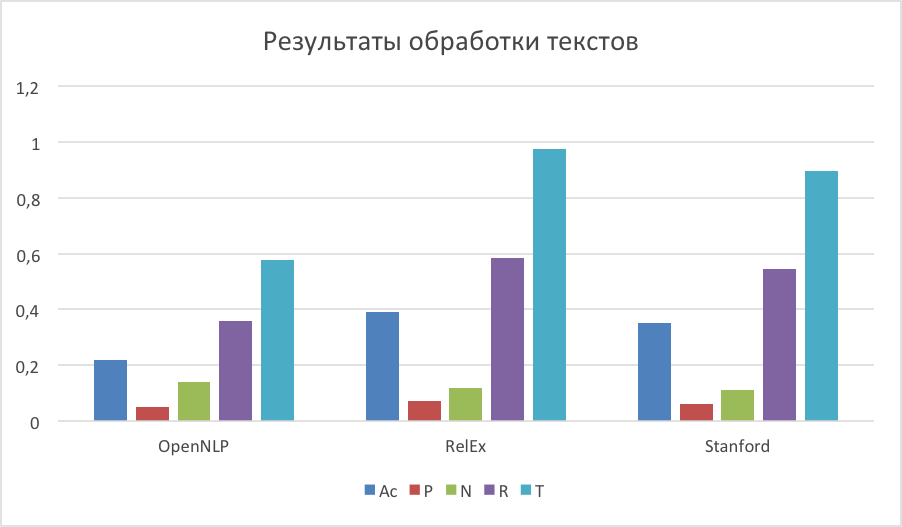
\includegraphics [scale=0.8] {ParserCompare}
  \caption{Результаты обработки текстов} 
  \label{img:ParserComp}  
\end{figure}

Из диаграммы видно, что наилучшее результаты показывает обработчик Relex\cite{OpenCogRelex}. После анализа необработанных инцидентов у всех обработчиков было выявлены проблемы двух типов:
\begin{enumerate}
	\item невозможность корректировки простых грамматических ошибок, связанных с пропущенными пробелами или неверным форматированием (ошибки первого типа);
	\item неверная интерпретация слов в предложении, например, слово please интерпретировалось как глагол, хотя является по смыслу "формой вежливости" (ошибки второго типа).
\end{enumerate}	\par

Несмотря на хорошие результаты~--- 63\% успешно разобранных предложений, ошибки первого и второго типа серьезно ухудшают результат. Эффективность разбора предложений в 63\% недостаточна для успешной работы системы. Чтобы улучшить показатель, был создан комплекс мер для устранения ошибок первого и второго типа.
	
 
\clearpage
\subsection{Исправление ошибок первого и второго типа} \label{sect2_2}
Чтобы исправить проблемы, связанные с ошибками первого и второго типа, была введена предварительная обработка текста, состоящая из 2-х фаз: комплексная корректировка для ошибок первого типа; обработка при помощи внутренней базы знаний для ошибок второго типа. 
Чтобы избавиться от орфографических, грамматических и синтаксических ошибок, был сконструирован составной корректировщик, который имеет модульную структуру и осуществляет корректировку последовательно (рис. 1.5). В результаты были сконструированы модули корректировки: Google API~--- модуль подключения к открытым системам Google для использования их алгоритмов корректировки; After the Deadline~--- модуль, использующий открытый программный продукт After the Deadline для исправления текстов; 

Таким способом удалось исправить большинство ошибок, связанный с синтаксисом, грамматикой и орфографией. Также удалось исправить ошибки неверного написания: наличия лишних пробелов, пропуска запятых и точек. Но по-прежнему осталась проблема обработки неверной интерпретации слов в тексте. \par

Для корректировки ошибок второго типа был сконструирован модуль для обработчика естественного языка Relex, который разбивал стандартный процесс обработки на «предобработку» и «обработку». Стадия «обработки» включает в себя алгоритм работы такой же как был до этого в модули, а стадия «предобработки» проверяет входные данные (слово или предложение) на предмет его вхождения во внутреннюю базу знаний и если таковое имеется, то приложение передает соответствующие корректировки обратно в модуль. Например, Relex во фразе "please install firefox" считает, что "please"~--- это глагол, поэтому базе знаний нашей системы отмечено, что "please"~--- это форма вежливости, тем самым Relex больше не интерпретирует "please" как глагол.

\clearpage
\subsection{Сравнение средств обработки русского и английского языков} \label{sect2_3}
Средства обработки естественного языка принято относить к большому классу средств NLP – Natural Language Processing \cite{NLP}. Для английского языка существует множество открытых средств обработки естественного языка, для русского языка найти их гораздо сложнее. Рассмотрим архитектуру средств обработки естественного языка на примере OpenCog Relex. \par
OpenCog Relex использует результаты работы открытого компонента для лексического анализа под названием Link Grammar \cite{linkgrammar}. Он поддерживает множество языков: английский, русский, турецкий, немецкий и т.д.  В качестве формата вывода Relex использует синтаксис Link Grammar и преобразует его в формат связей, как показано в примере 1. Разбор примера приводится далее. 

\textbf{Пример 1}. User is unable to start KDP web, please reinstall Java.\\
\textbf{Результат} 
\begin{verbatim}
		_obj(start, KBP)
pos(start, verb)
inflection-TAG(start, .v)
tense(start, present)
pos([web], WORD)
noun_number(KBP, singular)
definite-FLAG(KBP, T)
pos(KBP, noun)
_advmod(reinstall, please)
pos(reinstall, verb)
inflection-TAG(reinstall, .v)
tense(reinstall, present)
pos(please, adv)
inflection-TAG(please, .e)
noun_number(Java, singular)
definite-FLAG(Java, T)
pos(Java, noun)
pos(., punctuation)
_obj(,, Java)
pos(,, verb)
tense(,, infinitive)
HYP(,, T)
_to-do(unable, ,)
pos(unable, adj)
inflection-TAG(unable, .a)
tense(unable, present)
pos(to, prep)
inflection-TAG(to, .r)
pos(be, verb)
inflection-TAG(be, .v)
_predadj(User, unable)
noun_number(User, singular)
definite-FLAG(User, T)
pos(User, noun)

\end{verbatim}



Далее возьмем разбор слова start. В результате мы получаем несколько отношений:
\begin{itemize}
	\item pos(start, verb) - start глагол
	\item tense(start, present) - время настоящее
	\item inflection-TAG(start, .v) -  метод обозначения на схеме (индекс)
\end{itemize} \par
Остальные обработчики пока не поддерживают русский язык. Существуют открытые проекты, но они еще недостаточно развиты.
\section{Выводы}
В данной главе были рассмотрены существующие на данный момент интеллектуальные системы регистрации и анализа проблемных ситуаций, возникающих в ИТ-инфраструктуре предприятия.
 В таблице \ref{Comparsion} приведены сводные данные по системам. В главе также выработаны критерии сравнения обработчиков естественного языка и выполнен основной анализ обработчиков естественного языка. По показателям эффективности было решено использовать OpenCog Relex.

\begin{longtable}{|p{6cm}|p{0.5cm}|p{0.5cm}|p{0.5cm}|}
 \caption[Сравнительный анализ существующих решений]{Сравнительный анализ существующих решений}\label{Comparsion} \\ 
 \hline
 
 \multicolumn{1}{|c|}{\textbf{Сравнительный пункт}} & \multicolumn{1}{c|}{\textbf{HP Open View}} & \multicolumn{1}{c|}{\textbf{ServiceNOW}} & \multicolumn{1}{c|}{\textbf{IBM Watson}} \\ \hline 
\endfirsthead
\multicolumn{2}{c}%
{{\bfseries \tablename\ \thetable{} -- продолжение}} \\
\hline \multicolumn{1}{|c|}{\textbf{Сравнительный пункт}} & \multicolumn{1}{c|}{\textbf{HP Open View}} & \multicolumn{1}{c|}{\textbf{ServiceNOW}} & \multicolumn{1}{c|}{\textbf{IBM Watson}}  \\ \hline 
\endhead

\hline \multicolumn{2}{|r|}{{Продолжение следует}} \\ \hline
\endfoot

\hline \hline
\endlastfoot
\hline
   Мониторинг & Да & Да & Да \\
   \hline
   Регистрация инцидентов & Да & Да & Да\\
   \hline
   Управление системами & Да & Нет & Нет \\
   \hline 
   Создание цепи обработки (Workflow) инцидента & Да & Да & Нет \\
   \hline 
   Понимания и формализацию запросов на естественном языке & Нет & Нет & Да \\
   \hline 
   Поиск решений & Нет & Нет & Да \\
   \hline 
   Применение решений & Нет & Нет & Нет \\
   \hline
   Обучение решению инцидента & Нет & Нет & Да \\
   \hline
   Умение проводить логические рассуждения: генерализацию, специализацию, синонимичный поиск & Нет & Нет & Нет \\
   \hline
   
\end{longtable}
\clearpage
